\documentclass[conference]{IEEEtran}
\IEEEoverridecommandlockouts
\usepackage{booktabs}
\usepackage{multirow}
\usepackage{amsmath}
\usepackage{array}
\usepackage{url}
\usepackage{xcolor}
\usepackage{tikz}
\usetikzlibrary{arrows.meta,positioning,shapes.geometric,fit,calc}
\usepackage[hidelinks]{hyperref}

\definecolor{actitblue}{RGB}{21,75,121}
\definecolor{actitcyan}{RGB}{38,139,157}
\definecolor{actitgreen}{RGB}{52,133,91}
\definecolor{actitorange}{RGB}{210,121,34}
\definecolor{actitred}{RGB}{177,55,55}
\definecolor{actitgray}{RGB}{90,98,108}

\tikzset{
  box/.style={draw,rounded corners,align=center,minimum height=8mm,minimum width=18mm,font=\scriptsize,fill=white},
  flow/.style={-{Latex[length=2mm]},thick,draw=actitgray},
  trust/.style={draw=actitblue,dashed,rounded corners,inner sep=3mm},
  decision/.style={diamond,draw,align=center,aspect=2,font=\scriptsize,fill=white}
}

\title{From Observables to Actionable Intelligence:\\
An Evidence-Constrained Pipeline for Reducing Semantic\\
Over-Correlation in Cyber Threat Intelligence}

\author{\IEEEauthorblockN{Ammar Aikan, Alaaldeen AL-Shuwaie, and Munif AL-Omisi}
\IEEEauthorblockA{University of Science and Technology--Yemen\\
Sana'a, Republic of Yemen\\
Email address(es)---to be added before submission}}

\begin{document}
\maketitle

\begin{abstract}
Cyber threat intelligence (CTI) platforms routinely transform heterogeneous reports and telemetry into observables, entities, relationships, and exchange objects. Two shortcuts can undermine the resulting knowledge: treating every syntactically valid technical value as a malicious indicator, and creating semantic relationships from document-wide co-occurrence. This paper presents an evidence-constrained CTI pipeline, implemented in the ACTIT platform, that separates observed facts from detection claims and limits semantic relationships by context, entity type, and bounded pair generation. The system integrates 21 enabled registered sources, manual intake, internal sensors, privacy and relevance controls, deterministic deduplication, named entity recognition, observable extraction, correlation, PostgreSQL persistence, STIX 2.1 export, and optional unpublished MISP sharing. Its collection boundary applies redirect-aware server-side request forgery defenses, response and item bounds, fail-closed routing, review isolation, atomic export, and network separation. A retrospective production case study compares the stored graph before and after a conservative quality migration. Technical observables increased from 11,465 to 12,010 because validated IPv6, URL, domain, refanged IPv4, ASN, and MAC forms were recovered. Rule-generated relationships decreased from 74,173 to 21,462, a reduction of 52,711 (71.06\%). Semantic USES, TARGETS, and EXPLOITS relationships fell from 33,337 to 723, while the maximum semantic relationships generated for one event decreased from 4,990 to 46. A second preview reported no further changes, supporting idempotence of the migration. In addition, 291 external-source unit and integration tests passed in the audited worktree. These results establish structural correction and operational consistency, not an equivalent improvement in precision: the prepared 400-document, two-reviewer evaluation has not yet been adjudicated. The study contributes a reproducible architecture and an explicit evidence hierarchy for preventing unsupported CTI claims while retaining raw observations for analyst review.
\end{abstract}

\begin{IEEEkeywords}
cyber threat intelligence, observables, indicators, semantic relationships, STIX, MISP, data quality, SSRF, human-in-the-loop, ACTIT
\end{IEEEkeywords}

\section{Introduction}
Cyber threat intelligence systems ingest material from vulnerability databases, security advisories, news feeds, social sources, honeypots, authentication logs, and analyst submissions. Their value depends not only on collection breadth but also on the semantic discipline applied after collection. A syntactically valid IP address in a report may be malicious infrastructure, a benign example, a victim address, or an unrelated reference. Likewise, a threat actor and a tool appearing in the same long report are not sufficient evidence that the actor used that tool.

Two failure modes follow. First, \emph{observable escalation} turns a technical value into a malicious indicator without supporting evidence. Second, \emph{semantic over-correlation} creates relations from global co-occurrence and a trigger word, producing a dense but unreliable graph. Both errors can propagate to downstream exchange, correlation, visualization, and automated response.

STIX 2.1 distinguishes Cyber-observable Objects (SCOs), which represent observed facts, from higher-level intelligence objects and indicators \cite{oasis2021stix}. OpenCTI similarly separates observables and indicators and places imported knowledge into analyst workbenches when review is required \cite{openctiObservables,openctiWorkbench}. MISP supports structured sharing and analyst workflows, but a producer remains responsible for the semantics of the attributes it submits \cite{mispProject}. These models motivate a conservative rule: extraction confirms that a value occurs; it does not, by itself, establish maliciousness.

This paper presents an evidence-constrained pipeline implemented in ACTIT, an applied CTI platform. The design preserves observations, requires contextual or analyst evidence for stronger claims, and bounds relationship creation to local evidence and compatible types. It also treats collection as a security boundary: untrusted URLs, redirects, content, and dark-web inputs are constrained before they can enter central state.

We address four research questions:

\begin{itemize}
  \item \textbf{RQ1:} How can a CTI pipeline preserve technical observations without automatically asserting maliciousness?
  \item \textbf{RQ2:} How can relationship extraction reduce document-wide combinatorial over-correlation while retaining supported local relations?
  \item \textbf{RQ3:} What structural changes result when these controls are applied retrospectively to a live CTI database?
  \item \textbf{RQ4:} Which security and reliability controls are necessary around heterogeneous and manually supplied sources?
\end{itemize}

The contributions are: (1) an evidence hierarchy that separates syntax, context, enrichment, and analyst approval; (2) a context- and type-bounded relationship policy; (3) a secure multi-source ingestion architecture with atomic handoff and explicit trust boundaries; and (4) a production case study reporting pre/post structural measurements, idempotence, and clearly bounded validity claims.

\section{Background and Related Work}
\subsection{CTI Processing and Exchange}
CTI frameworks commonly organize work into collection, processing, analysis, storage, and dissemination. The framework by Spyros et al. combines heterogeneous collection, machine-learning enrichment, correlation, and MISP-based sharing \cite{spyros2025holistic}. ACTIT adopts this lifecycle but implements its own source adapters, central schema, processing pipeline, and deployment boundaries.

STIX 2.1 provides machine-readable SDOs, SCOs, SROs, and bundles \cite{oasis2021stix}. An SCO records an observed network or host fact, while an Indicator is a pattern intended to detect suspicious or malicious activity. Conflating the two causes a semantic error even if the underlying regex match is exact. Deterministic STIX identifiers additionally allow logically identical objects to converge rather than multiply across exports.

OpenCTI uses independently running connectors for external import, enrichment, analysis, and export \cite{openctiConnectors}. Its analyst workbench keeps proposed knowledge in a draft state until validation \cite{openctiWorkbench}. ACTIT uses a lighter connector boundary suitable for its deployment scale: collectors emit validated, versioned JSON; only the central backend writes authoritative CTI state. This preserves a single-writer boundary without claiming feature parity with OpenCTI.

\subsection{Data Quality and Human Review}
CTI quality includes provenance, relevance, timeliness, completeness, and confidence. Automated extraction is useful for scale, but confidence in pattern recognition is not equivalent to confidence that a value is malicious. ACTIT therefore retains uncertain records for review and uses human approval for stronger operational actions. This resembles draft/workbench patterns while remaining explicit about what has and has not been measured.

\subsection{Secure Web Collection}
Source collectors process attacker-controlled inputs. Server-side request forgery (SSRF) can exploit URL fetchers to reach loopback, link-local, or internal services. Redirects can invalidate a safe initial validation if destinations are not rechecked. Research on SSRF defenses emphasizes validation of URL components and redirect handling \cite{wessels2024ssrf}. ACTIT applies scheme, host, DNS/IP, port, path, redirect, size, and timeout constraints and fails closed when a structured route cannot be verified.

\section{System and Trust-Boundary Architecture}
Figure~\ref{fig:architecture} shows the implemented architecture. External Sources owns collection, privacy filtering, relevance classification, external-only deduplication, and versioned export. The gateway supplies a bounded delivery boundary for external snapshots and sensor pages. The Central Backend authenticates users, validates handoffs, executes extraction and analysis, and remains the only writer of authoritative PostgreSQL CTI state. MISP is an optional unpublished sharing/review copy, not the primary database.

\begin{figure*}[t]
\centering
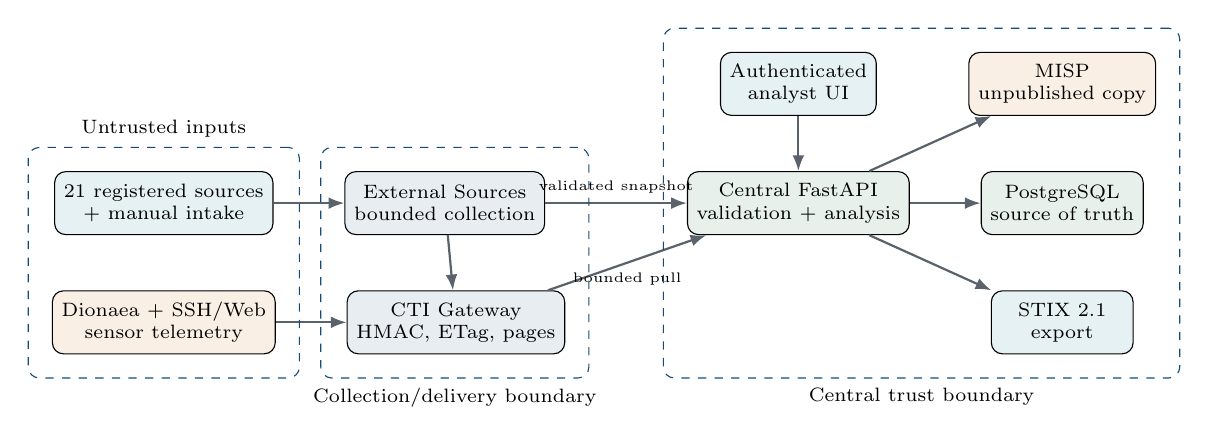
\begin{tikzpicture}[node distance=7mm and 9mm]
  \node[box,fill=actitcyan!12] (sources) {21 registered sources\\+ manual intake};
  \node[box,below=of sources,fill=actitorange!12] (sensors) {Dionaea + SSH/Web\\sensor telemetry};
  \node[box,right=of sources,fill=actitblue!10] (external) {External Sources\\bounded collection};
  \node[box,right=of sensors,fill=actitblue!10] (gateway) {CTI Gateway\\HMAC, ETag, pages};
  \node[box,right=18mm of external,fill=actitgreen!12,minimum width=25mm] (backend) {Central FastAPI\\validation + analysis};
  \node[box,right=of backend,fill=actitgreen!12] (db) {PostgreSQL\\source of truth};
  \node[box,above=of db,fill=actitorange!12] (misp) {MISP\\unpublished copy};
  \node[box,below=of db,fill=actitcyan!12] (stix) {STIX 2.1\\export};
  \node[box,above=of backend,fill=actitcyan!12] (ui) {Authenticated\\analyst UI};

  \draw[flow] (sources) -- (external);
  \draw[flow] (external) -- node[above,font=\tiny]{validated snapshot} (backend);
  \draw[flow] (external) -- (gateway);
  \draw[flow] (sensors) -- (gateway);
  \draw[flow] (gateway) -- node[below,font=\tiny]{bounded pull} (backend);
  \draw[flow] (ui) -- (backend);
  \draw[flow] (backend) -- (db);
  \draw[flow] (backend) -- (misp);
  \draw[flow] (backend) -- (stix);

  \node[trust,fit=(sources)(sensors),label={[font=\scriptsize]above:Untrusted inputs}] {};
  \node[trust,fit=(external)(gateway),label={[font=\scriptsize]below:Collection/delivery boundary}] {};
  \node[trust,fit=(backend)(db)(misp)(stix)(ui),label={[font=\scriptsize]below:Central trust boundary}] {};
\end{tikzpicture}
\caption{ACTIT architecture and principal trust boundaries. Pairwise internal networks restrict service reachability; only the central backend writes authoritative CTI state.}
\label{fig:architecture}
\end{figure*}

The production topology uses loopback publications for application services and explicit pairwise Docker networks. Containers use read-only roots where applicable, dropped Linux capabilities, \texttt{no-new-privileges}, resource bounds, and read-only secret/configuration mounts. Browser clients interact through the frontend's same-origin proxy and never receive gateway, collector, sensor, MISP, or database credentials.

\section{Evidence-Constrained Processing}
\subsection{Pipeline Stages}
Figure~\ref{fig:pipeline} presents the data path. Validation failures and privacy ambiguity are routed to review instead of silently entering accepted data. Canonical identities support incremental processing and provenance-preserving deduplication.

\begin{figure*}[t]
\centering
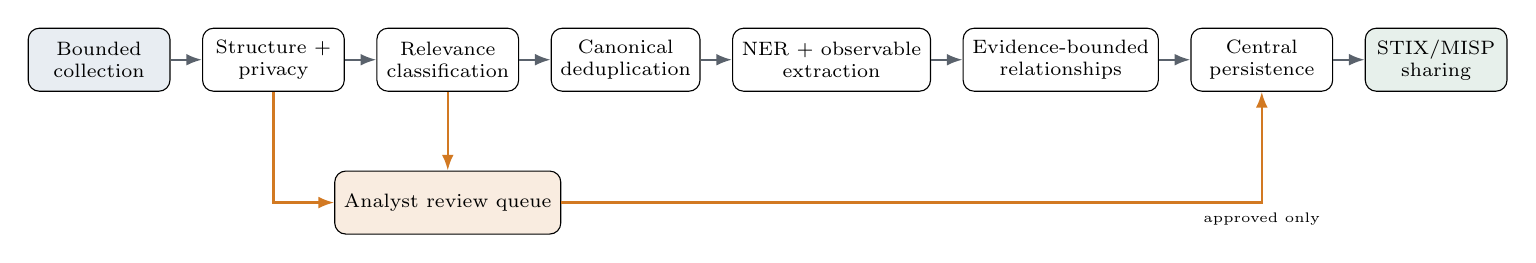
\begin{tikzpicture}[node distance=5mm and 4mm]
  \node[box,fill=actitblue!10] (collect) {Bounded\\collection};
  \node[box,right=of collect] (validate) {Structure +\\privacy};
  \node[box,right=of validate] (relevance) {Relevance\\classification};
  \node[box,right=of relevance] (dedup) {Canonical\\deduplication};
  \node[box,right=of dedup] (extract) {NER + observable\\extraction};
  \node[box,right=of extract] (relations) {Evidence-bounded\\relationships};
  \node[box,right=of relations] (store) {Central\\persistence};
  \node[box,right=of store,fill=actitgreen!12] (share) {STIX/MISP\\sharing};
  \node[box,below=10mm of relevance,fill=actitorange!14] (review) {Analyst review queue};

  \foreach \a/\b in {collect/validate,validate/relevance,relevance/dedup,dedup/extract,extract/relations,relations/store,store/share}
    \draw[flow] (\a) -- (\b);
  \draw[flow,draw=actitorange] (validate) |- (review);
  \draw[flow,draw=actitorange] (relevance) -- (review);
  \draw[flow,draw=actitorange] (review) -| node[below,font=\tiny]{approved only} (store);
\end{tikzpicture}
\caption{ACTIT evidence-constrained processing flow. Review and rejection artifacts remain separate from accepted datasets.}
\label{fig:pipeline}
\end{figure*}

\subsection{Observable--Indicator Evidence Hierarchy}
The pipeline distinguishes four evidence levels:

\begin{enumerate}
  \item \textbf{Syntactic evidence}: a validated parser or regex finds a correctly formed technical value.
  \item \textbf{Contextual evidence}: nearby text states the role or assessment of that value.
  \item \textbf{External evidence}: enrichment or a trusted source supports an operational assessment.
  \item \textbf{Human decision}: an authorized analyst approves the stronger claim or sharing action.
\end{enumerate}

Syntactic evidence creates an observable, not a malicious indicator. Figure~\ref{fig:gate} shows the decision logic. Extracted observables are exported as appropriate SCOs with deterministic identifiers. When maliciousness is unproven, MISP receives the value with \texttt{to\_ids=false}. Indicator creation requires a separate policy involving context, enrichment, source reliability, analyst approval, and lifecycle controls.

\begin{figure}[t]
\centering
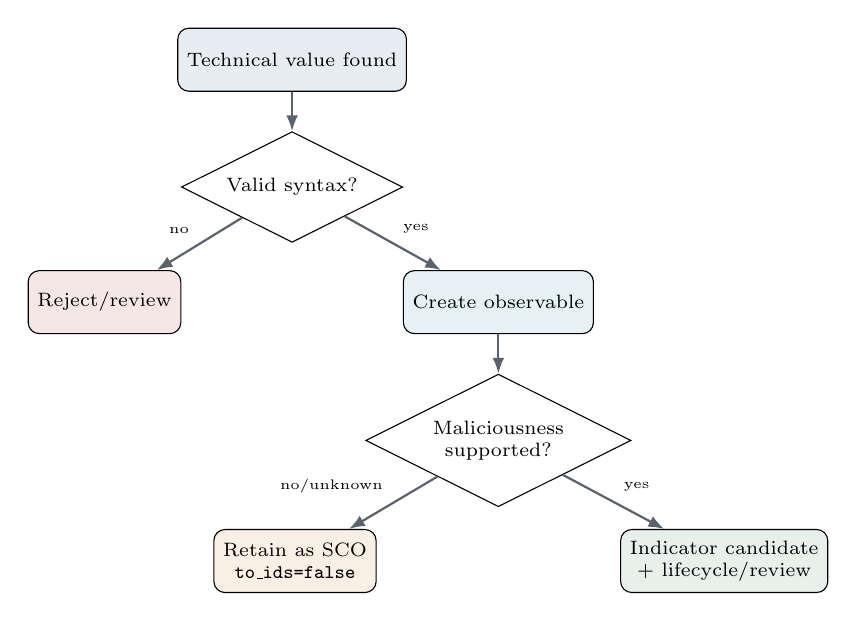
\begin{tikzpicture}[node distance=5mm]
  \node[box,fill=actitblue!10] (value) {Technical value found};
  \node[decision,below=of value] (valid) {Valid syntax?};
  \node[box,below left=7mm and 7mm of valid,fill=actitred!12] (reject) {Reject/review};
  \node[box,below right=7mm and 7mm of valid,fill=actitcyan!12] (obs) {Create observable};
  \node[decision,below=of obs] (evidence) {Maliciousness\\supported?};
  \node[box,below left=7mm and 7mm of evidence,fill=actitorange!12] (retain) {Retain as SCO\\\texttt{to\_ids=false}};
  \node[box,below right=7mm and 7mm of evidence,fill=actitgreen!12] (indicator) {Indicator candidate\\+ lifecycle/review};
  \draw[flow] (value) -- (valid);
  \draw[flow] (valid) -- node[above left,font=\tiny]{no} (reject);
  \draw[flow] (valid) -- node[above right,font=\tiny]{yes} (obs);
  \draw[flow] (obs) -- (evidence);
  \draw[flow] (evidence) -- node[above left,font=\tiny]{no/unknown} (retain);
  \draw[flow] (evidence) -- node[above right,font=\tiny]{yes} (indicator);
\end{tikzpicture}
\caption{Observable-to-indicator evidence gate. Extraction alone cannot assert maliciousness.}
\label{fig:gate}
\end{figure}

\subsection{Context-Bounded Relationships}
The earlier relationship rule searched an entire document for relation triggers and then paired compatible-looking entities globally. If $A$ actors and $T$ tools occur in one document, a single USES trigger can generate up to $A\times T$ candidate relations. Similar products arise for target and exploit types. Long reports therefore produce combinatorial graph density disconnected from local evidence.

The corrected policy segments text into sentences, maps extracted entities to sentence spans, and applies an allowlisted subject--predicate--object type matrix. USES, TARGETS, and EXPLOITS candidates require a relation trigger and compatible endpoints in the same sentence, with explicit pair caps. Negated or structurally unsupported candidates are not promoted. MENTIONS remains a provenance link rather than proof of a semantic action.

This rule is intentionally conservative. Cross-sentence coreference may contain true relations that the current extractor misses. The design prefers a reviewable false negative to an unsupported high-confidence edge in an operational graph.

\section{Secure Multi-Source Ingestion}
The committed registry contains 22 configured public-source definitions, 21 enabled during the audit. They cover RSS/news, CERT advisories, vulnerability databases, Reddit public feeds with bounded fallback, Hacker News queries, Telegram public previews, GitHub advisories, CISA KEV, and related structured sources. Operator-approved onion sources are stored outside version control and are not counted in the public registry total.

Manual intake is treated as untrusted. Public URLs pass scheme and credential checks, DNS resolution and private-address rejection, redirect revalidation, response-size and timeout bounds, content-type checks, and canonical routing. JSON intake accepts only bounded arrays or allowlisted collection keys. The analyst approves a proposed mapping bound to the preview hash; schema changes fail closed on recheck. Raw JSON is not returned to the browser.

Dark-web collection is GET-only through an explicit Tor SOCKS proxy. Enabled onion labels must be valid v3 identifiers, configured paths must remain within allowlists, and direct-web fallback is prohibited. Public API responses expose neither onion locations nor local artifact paths.

Each run creates a run-scoped dataset, review artifact, and manifest. Publication is atomic: a failed export preserves the previously validated latest export. Cancellation creates no new export. Stable URL/content identities deduplicate registered and manual observations without discarding provenance.

\section{Evaluation Method}
\subsection{Retrospective Production Audit}
The study uses a pre/post audit of ACTIT's PostgreSQL CTI state. The precondition contained 9,914 threat events: 9,895 external and 19 internal. It held 11,465 technical values, 41,520 total entities (41,501 from DNRTI extraction), 74,192 relationships, and nine correlations. The migration operated conservatively: it added validated observable forms, regenerated rule-based relations under the new policy, retained model entities, and preserved the 19 structured internal relationships.

A custom-format PostgreSQL backup preceded application. The maintenance service supports preview by default and requires explicit application. After migration, the same preview was executed again to test whether the operation converged. No training or new collection is included in these measurements.

\subsection{Verification Tests}
The audited worktree's external-source test suite was executed with Python's unittest discovery. It ran 291 tests in 21.775 seconds and passed. These tests cover connectors, preprocessing, privacy, manual URL security, JSON mapping, review decisions, export behavior, collection jobs, and REST integration. Passing tests demonstrate conformance to encoded requirements, not the absence of unknown vulnerabilities.

The repository contains additional backend, gateway, topology, deployment, frontend, and ML tests, but this paper reports only the freshly executed 291-test result to avoid combining heterogeneous historical counts.

\subsection{Prepared Human Evaluation}
A separate protocol sampled 400 documents from 9,887 unique eligible external texts across 39 strata after scanning 9,895 events and removing eight exact repeats. Two blinded reviewers are intended to annotate relevance, entities, observables, malicious/benign/unknown assessment, and USES/TARGETS/EXPLOITS relationships, followed by adjudication. All templates remain pending; therefore, this paper reports no human-ground-truth precision, recall, F1, or agreement result.

\section{Results}
\subsection{Observable Coverage}
Technical observables increased from 11,465 to 12,010 (+545). Conservative refanging and validation recovered 340 IPv6 occurrences, 85 URLs, 66 domains, 29 previously absent or defanged IPv4 occurrences, three ASNs, one MAC address, and other normalized values. This is an increase in syntactically validated coverage, not proof that the new values are malicious.

\subsection{Relationship Reduction}
Table~\ref{tab:relations} shows the structural effect. Rule-generated relations decreased by 52,711 (71.06\%). The three semantic relation types decreased from 33,337 to 723. The maximum semantic relation count for one event decreased from 4,990 to 46; no event produced 50 or more semantic relations after correction.

\begin{table}[t]
\caption{Relationship Counts Before and After Correction}
\label{tab:relations}
\centering
\small
\begin{tabular}{lrrr}
\toprule
Measure & Before & After & Change \\
\midrule
Rule-generated total & 74,173 & 21,462 & $-52,711$ \\
MENTIONS & 40,836 & 20,739 & $-20,097$ \\
EXPLOITS & 17,043 & 326 & $-16,717$ \\
TARGETS & 7,749 & 210 & $-7,539$ \\
USES & 8,545 & 187 & $-8,358$ \\
Semantic subtotal & 33,337 & 723 & $-32,614$ \\
Max semantic/event & 4,990 & 46 & $-4,944$ \\
\bottomrule
\end{tabular}
\end{table}

Figure~\ref{fig:bars} visualizes the relation-type changes on a logarithmic scale so that post-correction counts remain visible.

\begin{figure}[t]
\centering
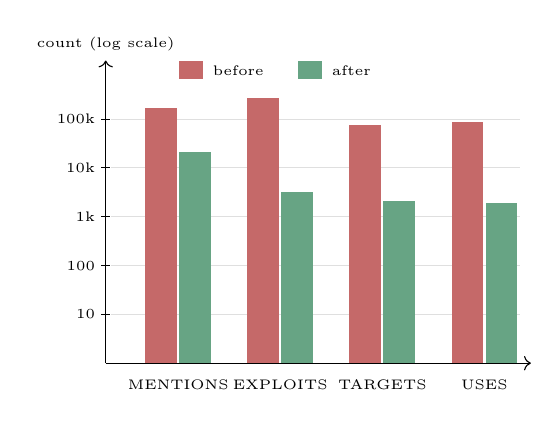
\begin{tikzpicture}[x=0.72cm,y=0.62cm]
  \draw[->] (0,0) -- (0,6.2) node[above,font=\tiny]{count (log scale)};
  \draw[->] (0,0) -- (7.5,0);
  \foreach \y/\lab in {1/10,2/100,3/1k,4/10k,5/100k}{
    \draw (-0.08,\y) -- (0.08,\y) node[left=2pt,font=\tiny]{\lab};
    \draw[gray!25] (0.1,\y) -- (7.3,\y);
  }
  % heights are 1 + log10(count), shifted for display
  \fill[actitred!75] (0.7,0) rectangle (1.25,5.236);
  \fill[actitgreen!75] (1.3,0) rectangle (1.85,4.316);
  \fill[actitred!75] (2.5,0) rectangle (3.05,5.431);
  \fill[actitgreen!75] (3.1,0) rectangle (3.65,3.513);
  \fill[actitred!75] (4.3,0) rectangle (4.85,4.889);
  \fill[actitgreen!75] (4.9,0) rectangle (5.45,3.322);
  \fill[actitred!75] (6.1,0) rectangle (6.65,4.932);
  \fill[actitgreen!75] (6.7,0) rectangle (7.25,3.272);
  \node[font=\tiny,align=center] at (1.28,-0.45) {MENTIONS};
  \node[font=\tiny,align=center] at (3.08,-0.45) {EXPLOITS};
  \node[font=\tiny,align=center] at (4.88,-0.45) {TARGETS};
  \node[font=\tiny,align=center] at (6.68,-0.45) {USES};
  \node[fill=actitred!75,minimum width=3mm,minimum height=2mm,label={[font=\tiny]right:before}] at (1.5,6.0) {};
  \node[fill=actitgreen!75,minimum width=3mm,minimum height=2mm,label={[font=\tiny]right:after}] at (3.6,6.0) {};
\end{tikzpicture}
\caption{Rule-generated relationship counts before and after correction. The vertical axis is logarithmic.}
\label{fig:bars}
\end{figure}

\subsection{Idempotence and Preservation}
The post-application preview returned \texttt{events\_changed=0}, \texttt{observables\_added=0}, and \texttt{rule\_relationship\_reduction=0}. The migration therefore reached a fixed point for the audited state. All 41,520 entities remained stored; 20,504 questionable entity occurrences were flagged for review rather than deleted. The 19 structured internal relationships were preserved.

\section{Discussion}
\subsection{Answers to the Research Questions}
\textbf{RQ1.} ACTIT preserves technical values as observables and decouples extraction certainty from maliciousness. Stronger indicator semantics require additional evidence and lifecycle policy. This prevents regex confidence from propagating as threat confidence.

\textbf{RQ2.} Sentence locality, endpoint-type constraints, trigger checks, and pair caps eliminate the global Cartesian-product behavior. The observed reduction is consistent with removal of structurally unsupported edges, but without adjudicated labels it is not a direct precision measurement.

\textbf{RQ3.} The migration increased validated observable coverage and substantially reduced relationship density while preserving entities and structured internal relations. Repeated preview confirmed idempotence for the audited state.

\textbf{RQ4.} Secure heterogeneous ingestion requires controls at URL selection, DNS resolution, redirects, content size/type, privacy review, export publication, authentication, and network reachability. A safe parser alone is insufficient when an attacker can redirect the collector or exploit an overprivileged service path.

\subsection{Operational Implications}
A smaller graph is not automatically a better graph. The benefit is traceability: an analyst can ask which sentence and typed endpoints justify an edge. The system retains raw observations and questionable entities instead of deleting them, allowing future reprocessing and human correction. This is important because an aggressive cleanup could hide evidence just as readily as an aggressive extractor invents it.

The collection/central split also limits authority. Collectors prepare a handoff but cannot write the authoritative database. ETag and stable identities allow unchanged snapshots to complete with zero reprocessing. Atomic latest-export replacement prevents a partial or failed run from becoming the current feed.

\section{Threats to Validity and Limitations}
\textbf{No completed human ground truth.} The most important limitation is that the 400-document annotation remains pending. The 71.06\% relation reduction must not be described as a 71.06\% accuracy improvement.

\textbf{Before/after confounding.} Observable normalization and relationship regeneration occur in one quality migration. The measurements describe a system-state transition, not an isolated randomized ablation.

\textbf{Conservative relation recall.} Same-sentence requirements miss valid cross-sentence and coreference relations. No coreference resolver or learned relation classifier is evaluated.

\textbf{Source and time dependence.} The database reflects ACTIT's enabled sources and collection period. Results may not generalize to other feeds, languages, or organizations.

\textbf{Test-suite scope.} The 291 passing tests validate encoded behavior with mocks and sanitized fixtures. They do not constitute penetration testing, formal verification, or live-source availability evidence.

\textbf{Indicator lifecycle remains incomplete.} ACTIT separates observables from indicators but does not yet implement a comprehensive source-reliability score, decay, revocation, and sighting policy comparable to mature CTI platforms.

\textbf{Deployment evidence.} Architecture claims are derived from source, deployment definitions, and recorded production verification. This study does not expose secrets or publish private operational artifacts. The paper does not claim that every repository option is enabled in production.

\section{Reproducibility and Ethics}
The evidence package should publish code revision, sanitized configuration schemas, source-registry summary, test command and output, migration logic, aggregate pre/post queries, and non-sensitive manifests. Private source lists, tokens, credentials, full collected texts, and analyst data must remain excluded. Dataset and article redistribution depends on source licenses and terms.

The implementation and paper avoid labeling an observable malicious without evidence. This reduces the risk of reputational or operational harm from unsupported attribution. Dark-web sources require explicit operator approval and are not disclosed. Collected text is treated as untrusted data, not instructions.

The authors intend to publish the paper, diagrams, evidence map, and legally redistributable artifacts through the ACTIT project website and the archive required by the selected venue. A permanent URL will be inserted only after the public package and licenses are verified.

\section{Conclusion}
This paper presented an evidence-constrained CTI pipeline that separates observed technical facts from malicious indicators, bounds semantic relationships to local typed evidence, and places secure controls around heterogeneous collection. In an ACTIT production case study, validated observable coverage increased while rule-generated relationships decreased by 71.06\%, the worst per-event semantic explosion fell from 4,990 to 46, and a repeated preview produced no additional changes. A fresh 291-test external-source suite passed.

These findings support structural correction, idempotence, and implementation conformance; they do not yet establish precision or recall improvement. Completing the blinded 400-document annotation is the next scientific step. Future work should report inter-annotator agreement, adjudicated per-source and per-type metrics, ablations of each constraint, cross-sentence relation models, source reliability, and indicator decay and revocation.

\section*{Acknowledgment}
The authors thank Dr. Raed Al-Dhabhani for supervising the ACTIT graduation project at the University of Science and Technology--Yemen. Additional funding or infrastructure acknowledgments will be added only after confirmation.

\bibliographystyle{IEEEtran}
\bibliography{references}
\end{document}
